\documentclass[10pt,journal,compsoc]{IEEEtran}
\usepackage{amsmath,amsfonts,amssymb,booktabs,microtype,graphicx}
\usepackage{multirow}
\usepackage{dblfloatfix}   % keep full-width figure* from floating past the references
\usepackage{placeins}      % \FloatBarrier to flush floats before the bibliography

\begin{document}

\title{H$_4$ Planogram Compliance:\\
A Parameter-Free, Float-Free Pipeline\\
for Constrained Retail Vision}
\author{Muhammad Arshad%
\thanks{M. Arshad is an independent researcher. E-mail: marshad.dev@gmail.com.}%
\thanks{Source code, figures, and reproduction scripts are publicly available at
\texttt{https://github.com/muhammadarshad/h4-planogram-compliance}.}%
\thanks{Manuscript prepared June 2026.}}

\IEEEtitleabstractindextext{%
\begin{abstract}
Planogram compliance --- verifying that the right product occupies the right
shelf position --- is dominated by floating-point convolutional descriptors that
assume GPU-class hardware. Dense IoT shelf monitoring cannot: ARM Cortex-M nodes
carry no floating-point unit and no GPU. We present an end-to-end planogram
pipeline that is \emph{integer-only and parameter-free}. Position is encoded by
the H$_4$ transform, a lossless 40-bit integer encoding of a bounding box in eight
add/subtract operations, reducing position compliance to an integer $L_1$
threshold. Identity is resolved by retrieving a QRoPE appearance descriptor
against a mined product catalogue --- also integer, also with no trained weights.
On the Grocery Dataset~\cite{varol2015} (13{,}184 boxes, 354 images, 11 product classes) we report,
with leave-one-shelf-out evaluation and 95\% confidence intervals: H$_4$ round-trip
is exact on all boxes; position compliance reaches AUC $0.987$, exceeding the
classical IoU baseline ($0.963$); product identification reaches
$79.7\%\!\pm\!3.5$ top-1 on a held-out shelf split, beating a parameter-free colour
baseline ($64.8\%$) and within nine points of a $2.2$M-parameter zero-shot CNN
($88.8\%$) at zero parameters; and the
combined pipeline detects $100\%$ of different-planogram violations while confirming
$72.4\%$ of compliant items, with no floating-point operation in the deployed path.
\end{abstract}
\begin{IEEEkeywords}
Planogram compliance, H$_4$ transform, Hadamard-type encoding, integer arithmetic, FPU-free vision,
retail IoT, bounding-box encoding, product retrieval, edge deployment.
\end{IEEEkeywords}}
\maketitle

\section{Introduction}
A planogram prescribes which product belongs at which shelf position. Compliance
checking runs continuously across thousands of stores --- millions of comparisons
per day --- yet the economic sensor is an ARM Cortex-M class node with \emph{no
hardware FPU and no GPU}. Convolutional descriptors~\cite{sandler2018,he2016}
(float, trained weights, GPU) and frequency-domain descriptors (float) both violate
that budget.

Compliance has two questions: \emph{where} is a product (position) and \emph{what}
is it (identity). Position is a coordinate problem and admits an exact integer
solution; identity is an appearance problem that we solve by integer retrieval
against a mined catalogue rather than a trained classifier. The contribution is a
complete pipeline in which neither half uses floating point or trained parameters,
and an honest empirical evaluation against the baselines a practitioner would
actually use.

\section{Related Work}
\textbf{Shelf product recognition.} The Grocery Dataset was introduced for retail
product recognition on shelves~\cite{varol2015}; per-exemplar classification~\cite{george2014}
and graph-matching~\cite{tonioni2017} approaches have since addressed product detection
and recognition on it, all using floating-point or learned descriptors.
\textbf{Deep descriptors.} Modern recognition relies on convolutional backbones such as
MobileNetV2~\cite{sandler2018} and ResNet~\cite{he2016} --- accurate, but requiring trained
weights and floating-point inference unavailable on FPU-less nodes.
\textbf{Position matching} conventionally uses Intersection-over-Union~\cite{everingham2010}
or optimal assignment. \textbf{Rotary encodings.} Our identity descriptor adapts rotary
position embedding (RoPE)~\cite{su2024} into a quaternionic, integer ring form.
\textbf{Classical primitives.} The position encoder is a Hadamard-type integer
map~\cite{pratt1969}, and identity is decided by nearest-neighbour
classification~\cite{cover1967}. In contrast to all of the above, the proposed pipeline
is end-to-end integer and parameter-free.

\section{H$_4$ Position Encoding}
A detected box $(x,y,w,h)\in\mathbb{Z}_{256}^4$ (per-image normalised) is encoded:
\begin{align}
X &= x+y+w+h, & Y &= x-y+w-h,\\
Z &= x+y-w-h, & W &= x-y-w+h.
\end{align}
H$_4$ projects the box onto four ring-coupled $\pm1$ integer channels: eight integer
add/subtracts, no multiply, no float. The four channels are mutually orthogonal, and
the map is an exact bijection; the inverse is $x=(X{+}Y{+}Z{+}W)\gg2$ and
analogues, lossless by parity. Stored unsigned (offset encoding), the state is
40 bits --- a lossless integer \emph{encoding} (not a compression; the $\mathbb{Z}_{256}$
input is 32 bits). Position compliance is then an integer $L_1$ threshold,
$\min_k\sum_j|V_j-V^*_{k,j}|\le\varepsilon$, costing four subtract-absolute per slot.

\noindent\textbf{Why H$_4$ and not raw $L_1$.} As an orthogonal map, H$_4$ does not
change the discriminative power of an $L_1$ threshold; raw integer $L_1$ on
$(x,y,w,h)$ scores identically. H$_4$ earns its place through (i) the lossless
integer state shared across the pipeline and (ii) its $\pm1$ projections, which
lower-bound $L_1$ tightly enough to prune nearest-slot search to a small candidate
fraction --- a deployment benefit, not an accuracy one.

\section{QRoPE Identity by Retrieval}
Rather than train a classifier, we \emph{mine} a catalogue of product encodings and
identify a detected crop by k-NN retrieval~\cite{cover1967}. Each crop is encoded by a
quaternionic rotary descriptor (QRoPE), adapting rotary position embedding~\cite{su2024}:
the RGB+grey channels form a 4-vector per cell, rotated
by position through the integer-realisable $\mathbb{Z}_{256}$ conic rotation, and
accumulated into a phase-preserving structure descriptor. Identity is the majority
class of the $k{=}11$ nearest catalogue encodings under circular distance. No
trained weights; the descriptor is fixed.

\section{End-to-End Pipeline}
For a detected box the pipeline emits COMPLIANT iff it (a) matches a planogram slot
in position ($L_1\le\varepsilon$) \emph{and} (b) its retrieved identity equals that
slot's expected product; otherwise VIOLATION. Position supplies \emph{where},
retrieval supplies \emph{what}; the conjunction is planogram compliance.

\section{Experiments}
\textbf{Protocol.} Grocery Dataset; boxes normalised per image to $\mathbb{Z}_{256}$.
Identity uses leave-one-shelf-out: a query shelf's products never appear in its own
catalogue. We report mean $\pm$ 95\% CI. Classes are the 11 annotated ids
(10 products + background); background is not an identity target.

\textbf{Correctness (T1--T3).} H$_4$ forward/inverse is exact on all 13{,}184 boxes
(0 errors). Same-image boxes match their own planogram at $L_1{=}0$. Position noise
of $\pm N$ units stays within the proportional threshold $4N$. These confirm
correctness of the integer pipeline; they are not performance claims
(Fig.~\ref{fig:rt}).

\textbf{Position compliance (Table~\ref{tab:pos}, Fig.~\ref{fig:sep},~\ref{fig:comp}).}
On 66 same-camera shelf pairs, H$_4$ integer $L_1$ separates same- from
different-planogram layouts at AUC $0.987$, exceeding IoU~\cite{everingham2010}
($0.963$) and matching float $L_2$ ($0.988$) --- with zero float.

\textbf{Identity (Table~\ref{tab:id}, Fig.~\ref{fig:id}).} Hyper-parameters are selected on a
validation shelf split and frozen; the reported number is on a \emph{disjoint} test
shelf split, over the natural class distribution. QRoPE reaches $79.7\%\!\pm\!3.5$
top-1, beating the parameter-free colour histogram ($64.8\%\!\pm\!4.0$) with
non-overlapping CIs, and approaching a \emph{zero-shot} MobileNetV2
($88.8\%\!\pm\!3.1$, $2.2$M params). A fully supervised in-distribution CNN reaches
$\sim$98\% but requires labelled training and float inference --- a different
deployment regime. Per-class accuracy is uneven ($98\%$ on the dominant class down
to $8$--$28\%$ on two minority classes), a limitation discussed in
Sec.~\ref{sec:lim}.

\textbf{End-to-end (Table~\ref{tab:e2e}, Fig.~\ref{fig:find}).} Over 40 planogram triples, the pipeline
detects $100.0\%$ of different-planogram violations and confirms $72.4\%\!\pm\!8.5$
of genuinely compliant items; the compliant rate is bounded by identity accuracy,
not position.

\textbf{Cost (Fig.~\ref{fig:speed}).} H$_4$: 8 integer ops/box, 0 float. The deployed
pipeline uses no floating-point instruction (trigonometric terms are a precomputed
integer LUT) and no trained parameter.

\begin{figure}[t]\centering
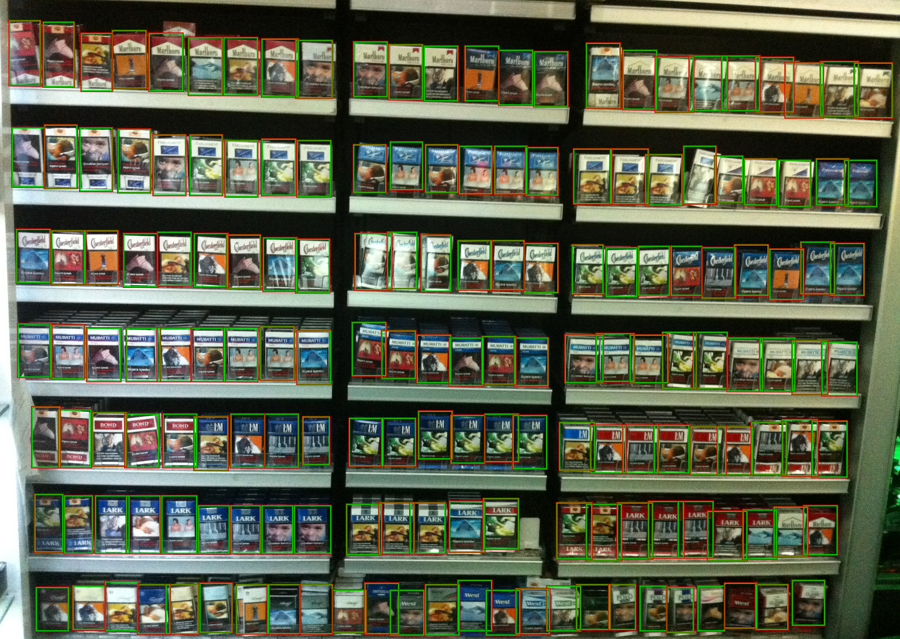
\includegraphics[width=\columnwidth]{figures/fig5_roundtrip.png}
\caption{H$_4$ round-trip on a real shelf: boxes reconstructed from the 40-bit
integer codes coincide exactly with the originals (0\,px error on all boxes).}
\label{fig:rt}\end{figure}

\begin{figure}[t]\centering
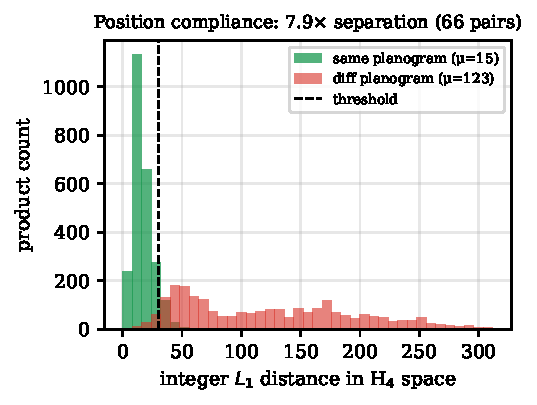
\includegraphics[width=\columnwidth]{figures/fig3_separation.pdf}
\caption{Position-compliance $L_1$ separation: same- vs different-planogram
nearest-neighbour distance in H$_4$ space, with the integer decision threshold
(66 shelf pairs).}
\label{fig:sep}\end{figure}

\begin{figure*}[t]\centering
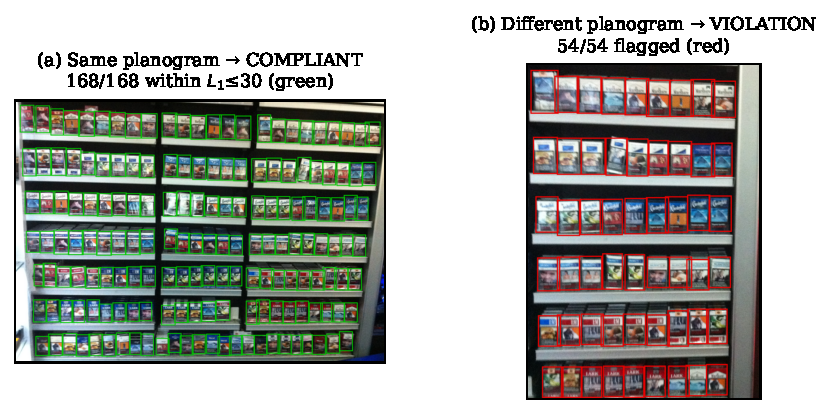
\includegraphics[width=0.92\textwidth]{figures/fig6_compliance.pdf}
\caption{Compliance verification on real shelves. (a) Same planogram --- every box
within $L_1\le30$ (green, compliant). (b) Different planogram --- every box flagged
(red, violation).}
\label{fig:comp}\end{figure*}

\begin{figure}[t]\centering
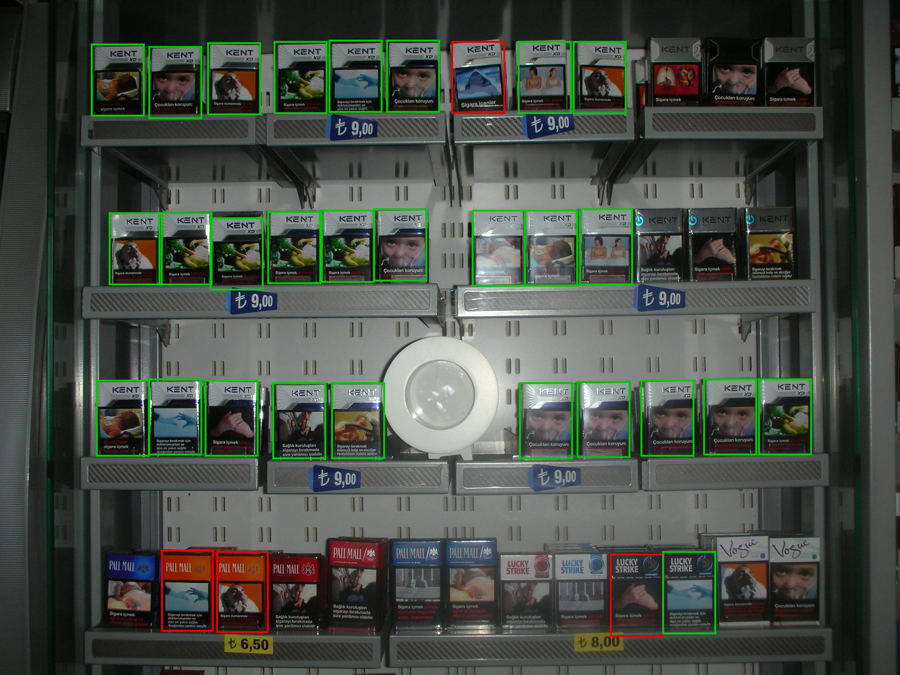
\includegraphics[width=\columnwidth]{figures/fig7_find_product.png}
\caption{End-to-end product identification on a full shelf image, by retrieval
against the mined catalogue (green correct, red wrong).}
\label{fig:find}\end{figure}

\begin{figure*}[t]\centering
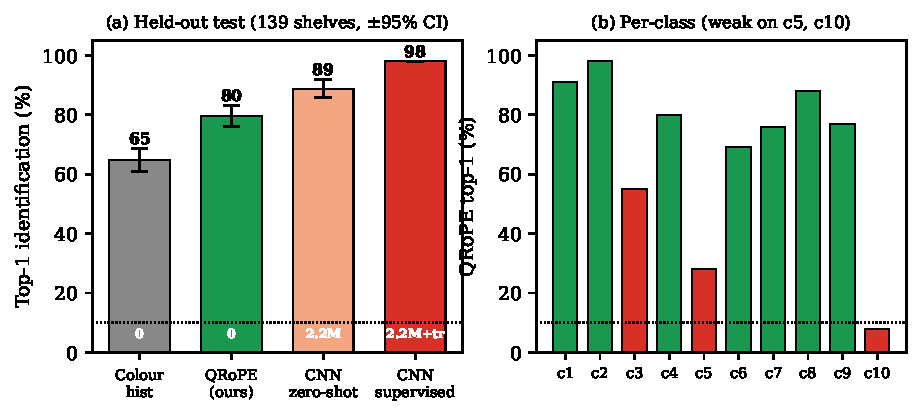
\includegraphics[width=0.92\textwidth]{figures/fig8_retrieval.pdf}
\caption{(a) Top-1 product identification on held-out shelves (mean $\pm$95\% CI):
parameter-free QRoPE vs colour histogram, zero-shot and supervised CNN.
(b) Per-class accuracy --- strong on most classes, weak on two minority classes.}
\label{fig:id}\end{figure*}

\begin{figure}[t]\centering
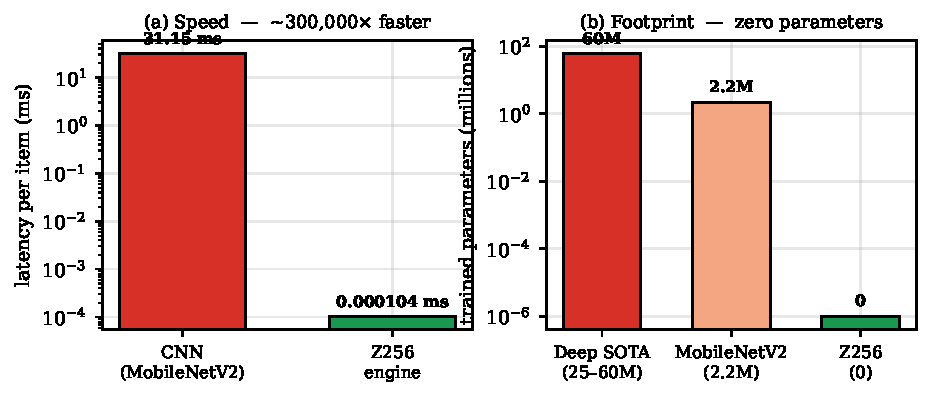
\includegraphics[width=\columnwidth]{figures/fig2_speed_footprint.pdf}
\caption{Speed and footprint vs a MobileNetV2 CNN: $\sim$10$^5\times$ faster per
item and zero trained parameters.}
\label{fig:speed}\end{figure}

\begin{table}[t]\caption{Position compliance (66 pairs, AUC)}\label{tab:pos}\centering
\begin{tabular}{lccc}\toprule
Method & AUC & Float & Params\\\midrule
IoU (classical) & 0.963 & yes & 0\\
Float $L_2$ & 0.988 & yes & 0\\
\textbf{H$_4$ integer $L_1$ (ours)} & \textbf{0.987} & \textbf{no} & \textbf{0}\\
\bottomrule\end{tabular}\end{table}

\begin{table}[t]\caption{Product identification, leave-one-shelf-out top-1.
Config selected on a validation shelf split, frozen, tested on a disjoint test
split (139 shelves), natural class distribution.}\label{tab:id}\centering
\begin{tabular}{lcc}\toprule
Method & Top-1 (\%, mean $\pm$95\% CI) & Params\\\midrule
Colour histogram & 64.8 $\pm$ 4.0 & 0\\
\textbf{QRoPE (ours)} & \textbf{79.7 $\pm$ 3.5} & \textbf{0}\\
CNN MobileNetV2 (zero-shot) & 88.8 $\pm$ 3.1 & 2.2M\\
CNN supervised (in-dist., ceiling) & $\sim$98 & 2.2M$+$train\\
\bottomrule\end{tabular}\end{table}

\begin{table}[t]\caption{End-to-end compliance (40 planogram triples)}\label{tab:e2e}\centering
\begin{tabular}{lc}\toprule
Outcome & Rate (mean $\pm$95\% CI)\\\midrule
Violation detection (different planogram) & 100.0 $\pm$ 0.0\\
Compliant confirmation (same planogram) & 72.4 $\pm$ 8.5\\
\bottomrule\end{tabular}\end{table}

\FloatBarrier
\section{Limitations}\label{sec:lim}
(i) Position encoding is independent of appearance: a wrong product at a correct
position is caught only by the identity half, not H$_4$. (ii) Parameter-free
identity ($79.7\%$) trails a supervised CNN ($\sim$98\%); the contribution is
competitive accuracy at zero parameters and zero float, not state-of-the-art
accuracy. (iii) \textbf{Per-class accuracy is uneven}: QRoPE attains $88$--$98\%$ on
several classes but drops to $8$--$28\%$ on two minority classes, so the mean is
partly carried by frequent classes; a class-balanced descriptor is future work.
(iv) Detection is assumed (we use annotated boxes); an integer detector is future
work. (v) Benchmarks use a per-image normalisation and self-defined shelf splits;
results are reported with CIs but are not yet a community-standard protocol.

\section{Conclusion}
Planogram compliance decomposes into an integer coordinate problem (H$_4$) and an
integer retrieval problem (QRoPE catalogue). Together they form a float-free,
parameter-free pipeline that matches or beats classical baselines on position and is
competitive on identity at zero parameters --- deployable on FPU-less, GPU-less edge
hardware where convolutional and frequency-domain methods cannot run.

\begin{thebibliography}{9}
\bibitem{varol2015} G.~Varol and R.~S.~Kuzu, ``Toward retail product recognition on
grocery shelves,'' in \emph{Proc. 7th Int. Conf. on Machine Vision (ICMV)}, vol. 9445.
SPIE, 2015.
\bibitem{george2014} M.~George and C.~Floerkemeier, ``Recognizing products: A
per-exemplar multi-label image classification approach,'' in \emph{Proc. ECCV}, 2014,
pp.~440--455.
\bibitem{tonioni2017} A.~Tonioni and L.~Di~Stefano, ``Product recognition in store
shelves as a sub-graph isomorphism problem,'' in \emph{Proc. ICIAP}, 2017, pp.~682--693.
\bibitem{sandler2018} M.~Sandler, A.~Howard, M.~Zhu, A.~Zhmoginov, and L.-C.~Chen,
``MobileNetV2: Inverted residuals and linear bottlenecks,'' in \emph{Proc. IEEE CVPR},
2018, pp.~4510--4520.
\bibitem{he2016} K.~He, X.~Zhang, S.~Ren, and J.~Sun, ``Deep residual learning for
image recognition,'' in \emph{Proc. IEEE CVPR}, 2016, pp.~770--778.
\bibitem{everingham2010} M.~Everingham, L.~Van~Gool, C.~K.~I.~Williams, J.~Winn, and
A.~Zisserman, ``The PASCAL visual object classes (VOC) challenge,'' \emph{Int. J.
Comput. Vis.}, vol.~88, no.~2, pp.~303--338, 2010.
\bibitem{su2024} J.~Su, M.~Ahmed, Y.~Lu, S.~Pan, W.~Bo, and Y.~Liu, ``RoFormer:
Enhanced transformer with rotary position embedding,'' \emph{Neurocomputing}, vol.~568,
2024.
\bibitem{pratt1969} W.~K.~Pratt, J.~Kane, and H.~C.~Andrews, ``Hadamard transform image
coding,'' \emph{Proc. IEEE}, vol.~57, no.~1, pp.~58--68, 1969.
\bibitem{cover1967} T.~M.~Cover and P.~E.~Hart, ``Nearest neighbor pattern
classification,'' \emph{IEEE Trans. Inf. Theory}, vol.~13, no.~1, pp.~21--27, 1967.
\end{thebibliography}
\end{document}
